%% LyX 2.3.6.1 created this file.  For more info, see http://www.lyx.org/.
%% Do not edit unless you really know what you are doing.
\documentclass[english]{article}
\usepackage[T1]{fontenc}
\usepackage[latin9]{inputenc}
\usepackage{geometry}
\geometry{verbose,tmargin=2.5cm,bmargin=2.5cm,lmargin=2.5cm,rmargin=2.5cm}
\usepackage{array}
\usepackage{calc}
\usepackage{textcomp}
\usepackage{multirow}
\usepackage{graphicx}

\makeatletter

%%%%%%%%%%%%%%%%%%%%%%%%%%%%%% LyX specific LaTeX commands.
%% Because html converters don't know tabularnewline
\providecommand{\tabularnewline}{\\}

\makeatother

\usepackage{babel}
\begin{document}

\section{9597 ALVL 2017}

\subsection{Paper 1}
\begin{enumerate}
\item \textbf{{[}NJC/PRELIM/9597/2017/P1/Q1{]} }

The head of the mathematics department would like to combine and rank
the examination results from 3 classes so that a summary report can
be generated. The mathematics teachers from these classes were instructed
to use the following format (on each line of a text file) when collating
the results: 
\noindent \begin{center}
<student index number>,<student examination score> 
\par\end{center}

After the results from each class had been collated, the following
was discovered. Each <student index number> was stored as a denary
value. However, the mathematics teachers stored <student examination
score> values using different base number systems.

The following were the base number systems utilised:
\begin{itemize}
\item Class 2A: binary 
\item Class 2B: octal
\item Class 2C: hexadecimal 
\end{itemize}
It should be noted that all index numbers and examination scores correspond
to non-negative integer values. 

\subsection*{Task 1.1 }

Write the program code for the function \texttt{base\_n\_to\_denary(value\_str,
n)}, which converts the given base \texttt{n}, non-negative integer
value, \texttt{value\_str}, into its corresponding denary value, and
then returns it. More specifically, this function should take the
following arguments. 
\begin{itemize}
\item \texttt{value\_str}: a string corresponding to a base n value. 
\item \texttt{n}: a positive integer between 2 and 16 corresponding to the
base number system used to represent \texttt{value\_str}. 
\end{itemize}
The function should then return an integer (i.e., a denary value),
whose value is equal to \texttt{value\_str}. You may not use any inbuilt
functionality to perform this conversion. 

\subsection*{Evidence 1}

The program code for the function \texttt{base\_n\_to\_denary(value\_str,
n)}.\hfill{} {[}3{]}

As mentioned above, the head of the mathematics department would like
to generate a summary report of the examination.

The format of this summary report is as follows: 

\noindent\fbox{\begin{minipage}[t]{1\columnwidth - 2\fboxsep - 2\fboxrule}%
\texttt{Mathematics results for classes 2A, 2B and 2C: }

\texttt{\bigskip{}
}

\texttt{The highest examination score: 100.0 }

\texttt{The average examination score: 50.0 }

\texttt{The lowest examination score: 0.0 }

\texttt{\bigskip{}
}

\texttt{The top 3 students are: }

\texttt{\bigskip{}
}

\texttt{Class Index Mark }

\texttt{2A ~~~1 ~~~~100}

\texttt{2C ~~~10 ~~~98 }

\texttt{2B ~~~3 ~~~~96 }%
\end{minipage}}

Note that the values used in the example summary report above are
not based on the actual values that are found in the given files.

\subsection*{Task 1.2}

Write the program code to perform the following. 
\begin{itemize}
\item Read and store the contents of the files: 
\begin{itemize}
\item \texttt{2A\_SCORES.TXT }
\item \texttt{2B\_SCORES.TXT}
\item \texttt{2C\_SCORES.TXT }
\end{itemize}
\item When storing this data, utilise the function \texttt{base\_n\_to\_denary(value\_str,
n)} to convert the scores in each file to their corresponding denary
values. 
\end{itemize}

\subsection*{Evidence 2 }

The program code to perform the above task.\hfill{} {[}3{]}

\subsection*{Task 1.3 }

Write the program code for the function sort\_student\_scores(\dots ),
which uses the class, index and score data (i.e., the data retrieved
from the 3 files listed in \textbf{Task 1.2}), and returns the same
information, but sorted in \textbf{descending order} based on score.

When considering the parameters and return value for sort\_student\_scores(\dots ),
your decision(s) should be based upon the usage of this information
to produce the summary report described earlier in this question.

Note that you are to utilise the \textbf{quicksort} algorithm to perform
the required sorting. Also note that you may not utilise any inbuilt
functionality to search or sort when writing this function.

\subsection*{Evidence 3 }

The program code for the function \texttt{sort\_student\_scores(\dots )}.
\hfill{}{[}5{]}

\subsection*{Task 1.4 }

Utilise the data from \textbf{Task 1.2}, and the function implemented
in \textbf{Task 1.3} -- i.e., \texttt{sort\_student\_scores(\dots )},
to produce the summary report described earlier in this question.

Note that you may not use any inbuilt functionality to find the: 
\begin{itemize}
\item Average score 
\item Maximum score
\item Minimum score 
\end{itemize}

\subsection*{Evidence 4 }

The program code to print the summary report.\hfill{} {[}3{]}

\subsection*{Evidence 5 }

A screenshot of the summary report output. \hfill{}{[}1{]}
\item \textbf{{[}NJC/PRELIM/9597/2017/P1/Q2{]} }

A Japanese restaurant would like to trial a new system for taking
orders. More specifically, the owners would like to trial a prototype
text-based system. You have been tasked to help with its implementation. 

The menu is currently stored in the text file \texttt{MENU.TXT}, with
each menu item stored on one line in the following format: 
\noindent \begin{center}
<menu item index number> <menu item name> <menu item price> 
\par\end{center}

Note that the 3 pieces of information are separated by spaces. The
<menu item index number> always contains 3 digits (including preceding
zeros), and the <menu item price> always begins with the \textquotedblleft \texttt{\$}\textquotedblright{}
sign.

Task 2.1 

Write the code to display and navigate through a text-based menu with
the following options: 
\noindent \begin{center}
\begin{tabular}{|l|}
\hline 
\texttt{1. Read menu data}\tabularnewline
\texttt{2. Take order }\tabularnewline
\texttt{3. Quit}\tabularnewline
\hline 
\end{tabular} 
\par\end{center}

You are to implement the following.
\begin{itemize}
\item Full functionality for Option 1 and Option 3.
\item A stub for Option 2. 
\end{itemize}
When implementing Option 1, take note of the following. 
\begin{itemize}
\item The menu items are to be read from \texttt{MENU.TXT}. 
\item For each menu item, the <menu item index number>, <menu item name>
and <menu item price> should be stored. You must implement an augmented
\textbf{linear search} (on <menu item index number>) to ensure that
insertions leave the menu items sorted in ascending order (i.e., by
finding the index of the element just greater than the search item).
\item The menu item index numbers in \texttt{MENU.TXT} need not be listed
in order, and there may be missing index numbers as certain old menu
items may have been omitted from the file. 
\end{itemize}
Also, the selection of Option 1 must precede the selection of Option
2, though Option 1 need only be selected once for each execution of
the menu program. Your implementation must incorporate these requirements.
Further, do ensure that proper exception handling is implemented for
user input.

\subsection*{Evidence 6 }

The program code for the text-based menu as specified above.\hfill{}
{[}8{]}

\subsection*{Task 2.2 }

Write the program code for Option 2. When Option 2 is selected (legally),
the following message should be displayed: 
\noindent \begin{center}
\begin{tabular}{|c|}
\hline 
\texttt{Please enter a menu item index (or \textminus 1 to complete
the order): }\tabularnewline
\hline 
\end{tabular}
\par\end{center}

The message is repeated for each <menu item index number> that is
input, and will repeat until the value \textminus 1 is input.

For each <menu item index number> that is input, a search should be
performed to ensure that it exists (based on the menu items read from
\texttt{MENU.TXT}). You are to implement the binary search algorithm
to perform this check. 

Note that for this sub-option, you need not implement any exception
handling. When an index that does not exist in \texttt{MENU.TXT} is
entered, the following message is to be output. Invalid menu index;
that index does not exist.

With each order, the user inputs one or more menu items (via <menu
item index>). Once all the ordered menu items have been entered, the
user then inputs -1 to conclude the order, at which point, the following
is output. 
\begin{itemize}
\item A list of all the ordered items -- for each item ordered, this includes:
(i) <menu item index number>, and (ii) the <menu item name>. 
\item The total price of all the items ordered. 
\end{itemize}
A sample of the above output would be as follows: 
\noindent \begin{center}
\begin{tabular}{|ll|}
\hline 
\texttt{Index} & \texttt{Item}\tabularnewline
\texttt{021} & \texttt{Ebi Curry}\tabularnewline
\texttt{064} & \texttt{California Temaki}\tabularnewline
\texttt{026} & \texttt{Salmon Fry Set}\tabularnewline
\texttt{127} & \texttt{Fried Chicken Ramen (Soup)}\tabularnewline
 & \tabularnewline
\multicolumn{2}{|l|}{\texttt{Total price : \$30.6}}\tabularnewline
\hline 
\end{tabular}
\par\end{center}

\subsection*{Evidence 7 }

The program code for Option 2. \hfill{}{[}7{]}
\item \textbf{{[}NJC/PRELIM/9597/2017/P1/Q3{]}}

Mickey is experimenting with object-oriented data structures, and
would like to implement a hybrid Linked List, where each node in the
Linked List is also the root of a Binary Search Tree. He intends to
utilise this hybrid structure to store integers ranging from 1 to
99. His design is as follows. 
\begin{center}
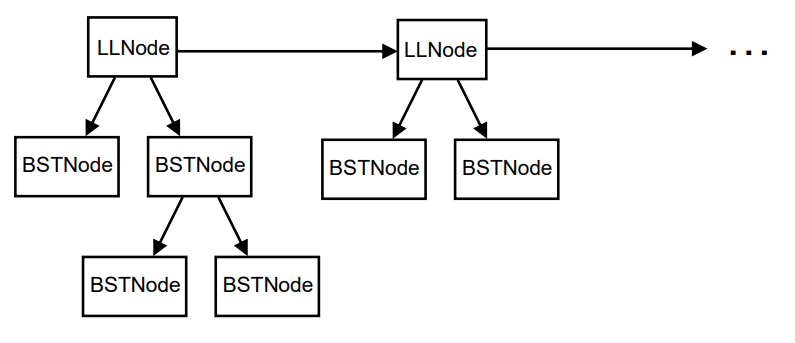
\includegraphics[width=0.5\paperwidth]{C:/Users/Admin/Desktop/Github/question_bank/LyX/static/img/9597-NJC-2017-P1-Q3-1}
\par\end{center}

\begin{center}
\texttt{}%
\begin{tabular}{|l|}
\hline 
\texttt{\hspace{0.25\columnwidth}BSTNode}\tabularnewline
\hline 
\texttt{-data: INTEGER}\tabularnewline
\texttt{-left: BSTNode}\tabularnewline
\texttt{-right: BSTNode}\tabularnewline
\hline 
\texttt{+constructor(INTEGER)}\tabularnewline
\texttt{+get\_data(): INTEGER}\tabularnewline
\texttt{+set\_data(INTEGER)}\tabularnewline
\texttt{+get\_left(): BSTNode}\tabularnewline
\texttt{+set\_left(BSTNode)}\tabularnewline
\texttt{+get\_right(): BSTNode}\tabularnewline
\texttt{+set\_right(BSTNode)}\tabularnewline
\texttt{+print()}\tabularnewline
\hline 
\multicolumn{1}{l}{\texttt{\hspace{0.25\columnwidth}$\uparrow$}}\tabularnewline
\hline 
\texttt{\hspace{0.25\columnwidth}LLNode}\tabularnewline
\hline 
\texttt{-next: LLNode}\tabularnewline
\hline 
\texttt{+constructor(INTEGER)}\tabularnewline
\texttt{+get\_next(): LLNode}\tabularnewline
\texttt{+set\_next(LLNode)}\tabularnewline
\hline 
\end{tabular}\texttt{~~~~~~~~~~~~}%
\begin{tabular}{|l|}
\hline 
\texttt{\hspace{0.25\columnwidth}HybridStructure}\tabularnewline
\hline 
\texttt{-first: LLNode}\tabularnewline
\hline 
\texttt{+constructor()}\tabularnewline
\texttt{+get\_first(): LLNode}\tabularnewline
\texttt{+set\_first(LLNode)}\tabularnewline
\texttt{+inLL(INTEGER)}\tabularnewline
\texttt{+contains(INTEGER)}\tabularnewline
\texttt{+insert(INTEGER)}\tabularnewline
\texttt{+print()}\tabularnewline
\hline 
\end{tabular}
\par\end{center}

Note that this Linked List is \textbf{singly-linked}, and also notice
that \textbf{each node of the Linked List} is \textbf{also the root
of a Binary Search Tree}. 

\subsection*{Task 3.1 }

Write the object-oriented code for the \texttt{BSTNode} and \texttt{LLNode}
classes described above. 

\subsection*{Evidence 8}

The program code for the \texttt{BSTNode} and \texttt{LLNode} classes.\hfill{}
{[}12{]}

Mickey\textquoteright s intention is to have the insert method from
the \texttt{HybridStructure} class act as follows. 
\begin{itemize}
\item When inserting integer \texttt{i }
\item First search the \textbf{Linked List} to determine if there exists
another integer \texttt{j} such that the tens digit in i and the tens
digit in \texttt{j} are the same
\item If the above is \texttt{True}, then insert integer \texttt{i} into
the \textbf{Binary Search Tre}e whose root Node holds the integer
\texttt{j}, else, insert integer \texttt{i} into the \textbf{Linked
List }
\end{itemize}
The following describes the functionality of the non-standard \texttt{HybridStructure}
methods.
\begin{itemize}
\item \texttt{+inLL(INTEGER)} : Returns \texttt{True} if the given integer
shares the same tens digit as another integer in the Linked List,
else returns \texttt{False}
\item \texttt{+insert(INTEGER)} : Inserts a new integer based on the procedure
described above 
\item \texttt{+contains(INTEGER)} : Returns \texttt{True} if the given integer
can be found in the structure, else returns \texttt{False}
\item \texttt{+print()} : Prints the contents of each Binary Search Tree
inorder, leaving a blank line in between each Linked List Node (and
the contents of its associated Binary Search Tree) 

For example, given the following \texttt{HybridStructure}: 
\begin{center}
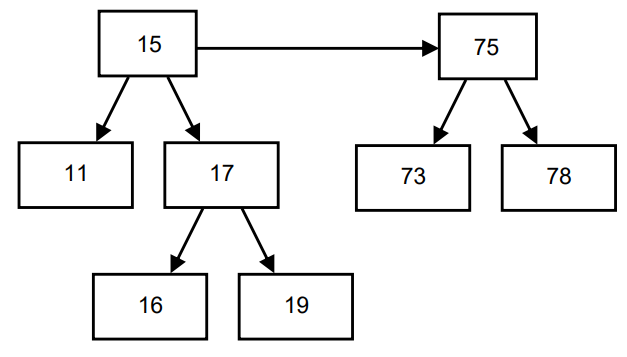
\includegraphics[width=0.5\paperwidth]{C:/Users/Admin/Desktop/Github/question_bank/LyX/static/img/9597-NJC-2017-P1-Q3-2}
\par\end{center}

The output would be: 

\noindent\fbox{\begin{minipage}[t]{1\columnwidth - 2\fboxsep - 2\fboxrule}%
11 

15 

16 

17 

19

73

75 

78%
\end{minipage}}
\end{itemize}

\subsection*{Task 3.2 }

Write the object-oriented code for the \texttt{HybridStructure} class
described above. 

\subsection*{Evidence 9 }

The program code for the \texttt{HybridStructure} class.\hfill{}
{[}25{]}

\subsection*{Task 3.3}

Initialise an instance of \texttt{HybridStructure}, insert the integers
\texttt{15 17 12 13 96 91 99 97} (in the order specified), and then
call the method \texttt{print()} to check its contents.

\subsection*{Evidence 10 }

The program code to for the above task.\hfill{} {[}2{]}

\subsection*{Evidence 11 }

The screenshot of the output. \hfill{}{[}1{]}
\item \textbf{{[}NJC/PRELIM/9597/2017/P1/Q4{]}}

Laura is always forgetting who she lends her books to and decides
to implement a special pair of Hash Tables to help her keep track
of her book loans. 

Laura has exactly 97 books, and has no plans to buy any new books. 

In her new system, a simple tuple (<Book Title>, <Person Who Borrowed
the Book>) is created each time she lends someone a book. 

In order for her system to work, she would like to implement two Hash
Tables: 
\begin{itemize}
\item The first Hash Table, \texttt{HT1}, utilises a Hash Function that
is applied to <Book Title>.
\item A checksum is applied to determine the Hash Value for each <Book Title>,
where the ASCII value of each character in the title is multiplied
by its position in the <Book Title> string (starting from left to
right), and then summed.
\item For example, given the <Book Title>: \textquotedblleft \texttt{A Cat}\textquotedblright ,
the summed value would thus be: 65\texttimes 1 + 32\texttimes 2 +
67\texttimes 3 + 97\texttimes 4 + 116\texttimes 5.
\item A \textbf{modulus operation} is then applied to determine the final
Hash Value.
\item The second Hash Table, \texttt{HT2}, utilises a similar Hash Function,
except that it is instead applied to <Person Who Borrowed the Book>. 
\end{itemize}

\subsection*{Task 4.1 }

Write the code for the function \texttt{get\_hash(my\_string)}, which
takes in a string argument and returns its resultant Hash Value, which
is defined by the checksum method described above. 

\subsection*{Evidence 12 }
\begin{itemize}
\item The program code for the \texttt{get\_hash(my\_string)} function.
\hfill{}{[}5{]}
\end{itemize}
In Laura\textquoteright s data structure design, the two Hash Tables,
HT1 and HT2, do not themselves store the loan information tuples --
i.e., (<Book Title>, <Person Who Borrowed the Book>). Instead, the
loan information tuples are stored in an array, \texttt{Loans}. 

The contents of \texttt{HT1} and \texttt{HT2} thus correspond to indices
of \texttt{Loans}. 

When a book is loaned, it is inserted into the next free index in
the array \texttt{Loans} (let this index be \texttt{k}), then, the
Hash Values for that particular loan are computed (based on <Book
Title> for \texttt{HT1} and <Person Who Borrowed the Book> for \texttt{HT2}),
and the value \texttt{k} stored in the relevant indices of \texttt{HT1}
and \texttt{HT2}. 

This is exemplified below. 
\begin{itemize}
\item Assume that we begin with no loans stored. 
\item Suppose that we then have a new loan: \texttt{(\textquotedblleft My
Book\textquotedblright , \textquotedblleft John Tan\textquotedblright )}
\item Assume that: 
\begin{itemize}
\item The Hash Value for \textquotedblleft \texttt{My Book}\textquotedblright{}
is \texttt{1} 
\item The Hash Value for \textquotedblleft \texttt{John Tan}\textquotedblright{}
is \texttt{3} 
\end{itemize}
\item Thus, to store this loan, we perform the following: 
\begin{itemize}
\item The new loan is stored in the Loans array via:

\texttt{Loans{[}0{]} = (\textquotedblleft My Book\textquotedblright ,
\textquotedblleft John Tan\textquotedblright ) }
\item Then, \texttt{0} is stored in \texttt{HT1{[}1{]}} (since the Hash
Value of \textquotedblleft \texttt{My Book}\textquotedblright{} is
\texttt{1}) 
\item And, \texttt{0} is also stored in \texttt{HT2{[}3{]}} (since the Hash
Value of \textquotedblleft \texttt{John Tan}\textquotedblright{} is
\texttt{3})
\end{itemize}
\item The resultant contents of \texttt{Loans}, \texttt{HT1} and \texttt{HT2}
would then be as follows.

\begin{tabular}{c|c|c|c|c|}
\cline{2-5} \cline{3-5} \cline{4-5} \cline{5-5} 
\texttt{Loans:} & \texttt{(\textquotedblleft My Book\textquotedblright , \textquotedblleft John
Tan\textquotedblright )} & \texttt{EMPTY} & \texttt{EMPTY} & \texttt{EMPTY}\tabularnewline
\cline{2-5} \cline{3-5} \cline{4-5} \cline{5-5} 
\texttt{HT1:} & \texttt{EMPTY} & \texttt{0} & \texttt{EMPTY} & \texttt{EMPTY}\tabularnewline
\cline{2-5} \cline{3-5} \cline{4-5} \cline{5-5} 
\texttt{HT2:} & \texttt{EMPTY} & \texttt{EMPTY} & \texttt{EMPTY} & \texttt{0}\tabularnewline
\cline{2-5} \cline{3-5} \cline{4-5} \cline{5-5} 
\end{tabular}
\end{itemize}
Laura has designed these Hash Tables to utilise the Closed Hashing
method of Linear Probing to resolve any conflicts that occur.

\subsection*{Task 4.2 }

By selecting appropriate Array and Hash Table sizes to suit Laura\textquoteright s
needs, write the code : 
\begin{itemize}
\item To initialise the array \texttt{Loans} and the two Hash Tables \texttt{HT1}
and \texttt{HT2}. 
\item For the function \texttt{insert(book\_title, person\_borrowing)},
which will \textquotedblleft insert\textquotedblright{} the given
loan into \texttt{Loans}, \texttt{HT1} and \texttt{HT2}. Note that
the function \texttt{get\_hash(my\_string)}, which was implemented
for \textbf{Task 4.1}, should be used. 
\end{itemize}

\subsection*{Evidence 13 }

The program code to initialise \texttt{Loans}, \texttt{HT1} and \texttt{HT2},
and the code for the function \texttt{insert(book\_title, person\_borrowing}.
\hfill{}{[}10{]}

\subsection*{Task 4.3 }

Write the code for the functions: 
\begin{itemize}
\item \texttt{find\_loan\_by\_title(title)}, which returns the loan tuple
corresponding to the \texttt{title} given, or else, will return an
empty tuple.
\item \texttt{find\_loan\_by\_person(person)}, which returns the loan tuple
corresponding to the \texttt{person} given, or else, will return an
empty tuple.
\item \texttt{remove\_loan\_by\_title(title)}, which deletes the loan tuple
corresponding to the \texttt{title} given and returns \texttt{True},
or else, returns \texttt{False} if it was not removed. This should
also remove the corresponding entries in \texttt{HT1} and \texttt{HT2}. 
\item \texttt{remove\_loan\_by\_person(person)}, which deletes the loan
tuple corresponding to the \texttt{person} given and returns \texttt{True},
or else, returns \texttt{False} if it was not removed. This should
also remove the corresponding entries in \texttt{HT1} and \texttt{HT2}. 
\end{itemize}
Ensure that you practice good \textbf{modularity} and \textbf{code
reuse} when implementing these functions. 

\subsection*{Evidence 14}
\begin{itemize}
\item The program code to for the above mentioned functions. \hfill{}{[}12{]}
\end{itemize}

\subsection*{Task 4.4 }

Write code to modify the \texttt{insert(book\_title, person\_borrowing)}
function such that it prints the amount of additional probing that
is required on any insertion -- i.e., prints the number of iterative
steps that linear probing was required to perform in order to find
an insertion point. 

\subsection*{Evidence 15 }
\begin{itemize}
\item The program code to that is required to make the above mentioned modification.
\hfill{} {[}3{]}
\end{itemize}
\end{enumerate}

\section{9597 ALVL 201X TEMPLATE}
\noindent \begin{center}
\begin{tabular}{c|l|}
\cline{2-2} 
\multirow{2}{*}{\texttt{In{[}1{]}:}} & \texttt{\# Task 1.1}\tabularnewline
 & \texttt{Program Code}\tabularnewline
\cline{2-2} 
\multirow{2}{*}{\texttt{In{[}2{]}:}} & \texttt{\# Task 1.2}\tabularnewline
 & \texttt{Program Code}\tabularnewline
\cline{2-2} 
\multirow{2}{*}{\texttt{In{[}3{]}:}} & \texttt{\# Task 1.3}\tabularnewline
 & \texttt{Program Code}\tabularnewline
\cline{2-2} 
\multicolumn{1}{c}{} & \multicolumn{1}{l}{\texttt{Output:}}\tabularnewline
\end{tabular}
\par\end{center}

\noindent\fbox{\begin{minipage}[t]{1\columnwidth - 2\fboxsep - 2\fboxrule}%

\subsubsection*{Task X.X}

\hfill{}

\subsubsection*{Evidence X}%
\end{minipage}}

\noindent %
\noindent\begin{minipage}[t]{1\columnwidth}%
\texttt{FUNCTION CalCheckDigit(Number AS STRING, Total AS INTEGER)
RETURNS STRING}

\texttt{\qquad{}IF LENGTH(Number) > 1 THEN}

\texttt{\qquad{}\qquad{}Digit <- INTEGER(LBFT(Number,1))}

\bigskip{}

\texttt{// Calculate ISBN, an example of how the function is called.}

\texttt{// Second parameter is always 0.}

\texttt{ISBN = CalCheckDigit(\textquotedbl 184146208\textquotedbl ,0)}%
\end{minipage}
\begin{enumerate}
\item {} 
\begin{center}
\begin{tabular}{|l|l|l|}
\hline 
\multicolumn{3}{|c|}{\texttt{Class: Connection Node}}\tabularnewline
\hline 
\multicolumn{3}{|c|}{Attributes}\tabularnewline
\hline 
\texttt{\hspace{0.01\columnwidth}}Identifier & \texttt{\hspace{0.01\columnwidth}}Data Type & \texttt{\hspace{0.05\columnwidth}}Description\tabularnewline
\hline 
\texttt{DataValue} & \texttt{STRING} & The node data\tabularnewline
\hline 
\texttt{LeftChild} & \texttt{INTEGER} & The left node pointer\tabularnewline
\hline 
\texttt{RightChild} & \texttt{INTEGER} & The right node pointer\tabularnewline
\hline 
\end{tabular}
\par\end{center}
\item {}
\begin{center}
\begin{tabular}{|l|}
\hline 
\texttt{\hspace{0.25\columnwidth}ToDo}\tabularnewline
\hline 
\texttt{category : STRING}\tabularnewline
\texttt{description : STRING}\tabularnewline
\hline 
\texttt{constructor(c : STRING, d : STRING)}\tabularnewline
\texttt{set\_category(s : STRING)}\tabularnewline
\texttt{set\_description(s : STRING)}\tabularnewline
\texttt{get\_category() : STRING}\tabularnewline
\texttt{get:\_description() : STRING}\tabularnewline
\texttt{summary() : STRING}\tabularnewline
\hline 
\end{tabular}
\par\end{center}
\item {}
\noindent \begin{center}
<INSERT\_IMAGE\_HERE>
\par\end{center}
\item {}

\begin{tabular}{lccccccccccccccccccccccccccc}
\textbf{Plain text alphabet:} & \texttt{a} & \texttt{b} & \texttt{c} & \texttt{d} & \texttt{e} & \texttt{f} & \texttt{g} & \texttt{h} & \texttt{i} & \texttt{j} & \texttt{k} & \texttt{l} & \texttt{m} & \texttt{n} & \texttt{o} & \texttt{p} & \texttt{q} & \texttt{r} & \texttt{s} & \texttt{t} & \texttt{u} & \texttt{v} & \texttt{w} & \texttt{x} & \texttt{y} & \texttt{z} & \tabularnewline
 & \texttt{$\downarrow$} &  &  & \texttt{$\downarrow$} &  &  &  &  &  &  &  &  &  &  &  &  &  &  &  &  &  &  &  &  &  & \texttt{$\downarrow$} & is substituted by\tabularnewline
\textbf{Cipher text alphabet:} & \texttt{A} & \texttt{P} & \texttt{L} & \texttt{E} & \texttt{B} & \texttt{C} & \texttt{D} & \texttt{F} & \texttt{G} & \texttt{H} & \texttt{I} & \texttt{J} & \texttt{K} & \texttt{M} & \texttt{N} & \texttt{O} & \texttt{Q} & \texttt{R} & \texttt{S} & \texttt{T} & \texttt{U} & \texttt{V} & \texttt{W} & \texttt{X} & \texttt{Y} & \texttt{Z} & \tabularnewline
\end{tabular}
\end{enumerate}

\end{document}
